{$\space$\par}
\vspace{0.5cm}
\justifying
\section*{{\bfseries \LARGE Questão 8 -} {\bfseries \large Tasse et al. (2011) mediu a emissão de raios x em AGNs para estudar a relação entre a atividade do AGN e a taxa de formação estelar na galáxia hospedeira. Seus dados se encontram no arquivo xrays\_tasse.tsv. As colunas são nome do AGN (Name), log fluxo em raios X moles (logFxs), log fluxo em raios X duros (logFxh), magnitudes gmag, rmag e imag, desvio para o vermelho (zph), logaritmo da massa da galáxia (logM) e logaritmo da taxa de formação estelar (logSFR).}}

\vspace{0.3cm}

\begin{enumerate}
    \item Faça um gráfico de logFxs versus logFxh. Sobreponha a este gráfico as seguintes curvas de regressão, cada uma com cor diferente: OLS, regressão quantílica da mediana, estimador de Nadaraya-Watson e LOESS.
        
    \item Represente a densidade do espaço logM versus logSFR usando um histograma bidimensional e curvas de contorno.
\end{enumerate}

\vspace{0.8cm}

\begin{figure}[h]
    \centering
    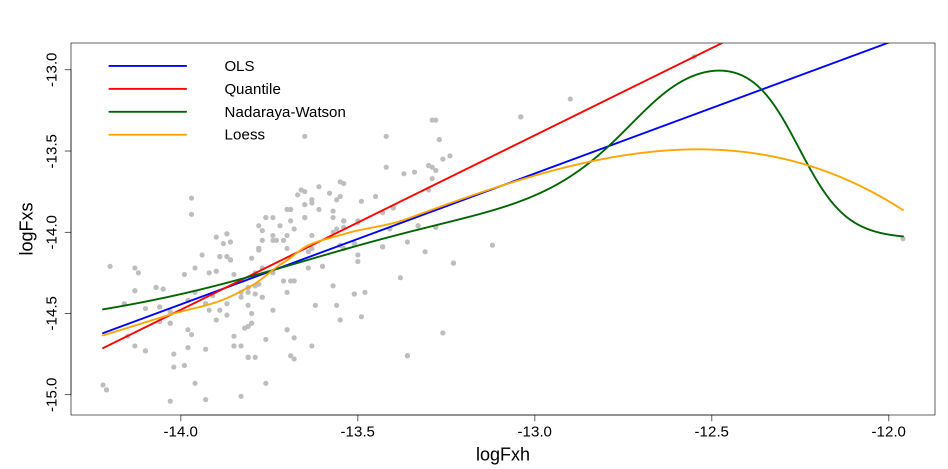
\includegraphics[width=0.8\linewidth]{Figuras/fits.png}
    \caption{Dados do fluxo de raios-X moles vs duros. As linhas representam diferente tipos de regressões aplicadas nos dados.}
    \label{fig:enter-label}
\end{figure}

\textcolor{red}{Ao realizar uma regressão podemos escolher diferentes tipos de estimadores e sua escolha dependerá da natureza do problema. Neste cenário, vemos que a regressão local e a regressão usando o estimador de Nadaraya-Watson foram mais suscetíveis aos objetos nos extremos das distribuições, podendo gerar problemas de 'overfitting'.}

\vspace{2em}

\begin{lstlisting}
    # Data
    agns = read.table('/content/xrays_tasse.tsv', header=T, sep='|')
    agns = agns[complete.cases(agns),]
    
    # Packages
    install.packages('quantreg')
    library(quantreg)
    install.packages("np")
    library(np)
    
    # Fitting
    fit_ols = lm(logFxs ~ logFxh, data = agns)
    fit_qtl = rq(logFxs ~ logFxh, data = agns, tau = 0.5)
    fit_nw = npreg(logFxs ~ logFxh, data = agns, bws = 0.2)
    fit_loe = loess(logFxs ~ logFxh, data = agns)
    
    # Points
    x = seq(min(agns$logFxh), max(agns$logFxh), length.out = 200)
    x_df = data.frame(logFxh = x)
    
    # Plotting
    options(repr.plot.width=16, repr.plot.height=8)
    plot(agns$logFxh, agns$logFxs, pch=19, col='gray', xlab='logFxh', ylab='logFxs',
     cex.lab=1.8, cex.axis=1.5)
    lines(x, predict(fit_ols, newdata = x_df), col='blue', lwd=3)
    lines(x, predict(fit_qtl, newdata = x_df), col='red', lwd=3)
    lines(x, predict(fit_nw, exdat = x_df), col='darkgreen', lwd=3)
    lines(x, predict(fit_loe, newdata = x_df), col='orange', lwd=3)
    legend('topleft', legend=c('OLS', 'Quantile', 'Nadaraya-Watson', 'Loess'), 
    col=c('blue','red','darkgreen','orange'), lwd=3, cex=1.5, bty='n')
\end{lstlisting}

\begin{figure}[h]
    \centering
    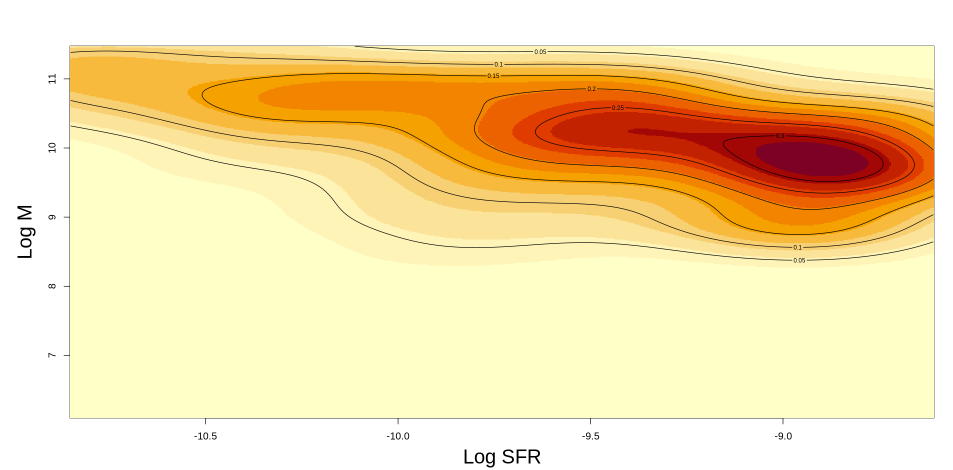
\includegraphics[width=0.8\linewidth]{Figuras/hist_2d.png}
    \caption{curvas de contorno com histograma 2D da massa da galáxia versus formação estelar, ambos em logaritmo.}
    \label{hist_2d}
\end{figure}


\textcolor{red}{b) Para representar a densidade bidimensional usei kernels gaussianos, onde cada ponto receberá uma distribuição gaussiana 2D com certa largura e ao final todas distribuições serão levadas em conta no histograma 2D. Percebe-se que galáxias com uma baixa taxa de formação estelar são geralmente mais massivas. Isso pode ser explicado pela evolução de galáxias, onde as galáxias mais massivas são elípticas vermelhas que já estão velhas e sem formação de estrelas, enquanto as galáxias de menor massa possuem maior formação estelar e são mais jovens. }

\begin{lstlisting}
    kde = kde2d(agns$logSFR, agns$logM, n=500)
    image(kde, xlab='Log SFR', ylab='Log M', cex.lab=2)
    contour(kde,add=T)
\end{lstlisting}

